\documentclass[10pt,conference,compsocconf]{IEEEtran}

%\usepackage{times}
%\usepackage{balance}
\usepackage{url}
\usepackage{graphicx}	% For figure environment
\usepackage{subcaption}
\usepackage{cite}

\begin{document}
\title{Computational Intelligence Lab Project:\\ Road Segmentation}

\author{
  Igor Pesic\\
  Department of Computer Science,\\ ETH Zurich
  \and
  Felipe Sulser\\
  Department of Computer Science,\\ ETH Zurich
  \and
  Minesh Patel\\
  Department of Computer Science,\\ ETH Zurich
}

\maketitle

\begin{abstract}
  Image segmentation of aerial road images has gained significant research
  interest in recent years due to numerous applications ranging from civil
  infrastructure to disaster preparation. In this work, we focus specifically
  on road segmentation, which is a simpler, but still very useful, subset of
  the general problem. Our goal is to accurately classify image pixels as part
  of either a road or the background. To this end, we have combined techniques
  proposed in several academic research papers and have tailored them to suit
  our requirements and resources as best as possible. Our solution uses a
  convolution neural network (CNN) in addition to techniques for data
  augmentation, feature selection, and post-processing. We find that our
  results are close to those of state-of-the-art solutions in current academic
  work despite our model being much simpler.
\end{abstract}

\section{Introduction}

Image segmentation covers a general class of problems that require classifying
input images' pixels into different regions, called \emph{segments}, based on
predefined criteria.  \emph{Road segmentation} is a subset of image
segmentation that focuses on identifying all image pixels belonging to roads
and has gained academic interest due to numerous real-world applications
ranging from automated monitoring of civil
infrastructure~\cite{radopoulou2016improving} to disaster
preparedness~\cite{li2007fuzzy}. 

Our goal in this work is to perform accurate road segmentation on aerial
satellite images. Given a set of input aerial images, we would like to
accurately determine which pixels belong to roads and which do not, assigning
each pixel a value of 0 (no road) or 1 (road). Ideally, we would segment the
images at a pixel granularity, but in order to simplify the problem, we use an
approach that achieves patch-wise granularity. We find that our approach
simplifies the problem substantially and is sufficient for this course
project. 

Our solution makes use of a convolutional neural network (CNN) combined with
pre- and post-processing steps in order to achieve high-accuracy road
segmentation.  To the best of our knowledge, we have designed a novel
architecture, which combines multiple academic works on similar
topics~\cite{mthesis,Mnih2010,vgg,xavier} and extends the combination by adding
our own ideas. Although we focused primarily on the design of our CNN, we also
invested a substantial amount of effort into post-processing the outputs using
a denoising step in order to improve the final results.

This report has the following structure: in Section \ref{sec:Data} we explain
the preprocessing we do before training and evaluating the model. In Section
\ref{sec:model_and_methods} we describe our model, including both the CNN and
the denoising applied afterwards. Finally, in \ref{sec:results} we discuss the
results we achieve using our model.


\section{Data}
\label{sec:Data}

\subsection{Data Augmentation}
\label{sec:data_aug}
The input data set consists of 100 labeled aerial images of road maps. Since
our approach uses a deep neural network, we need a large amount of input data
with which to train the model. Therefore, we expand the input data set by also
training with transformed versions of the provided images. To generate the
transformed images, we rotate each input image by 90 degrees and mirror it. In
addition to increasing the training data set size, this approach also makes our
model more robust by training with roads of different orientations than just
the ones provided in the input data set. 

Additionally, we observed that the model's predictions on diagonal roads were
far less accurate than on horizontal and vertical ones. We attributed this
to the lack of diagonal roads in our original training data set. In order to
fix this, we selected 9 images with diagonal roads and highways, which we
rotate again by 180 and 270 degrees and add to the training data set. This
allows our model to more accurately segment diagonal roads during prediction.

Finally, we observed inconsistencies in the labeling of some images in the
input dataset (i.e., a building classified as a road and vice-versa), and we
decided to discard those inputs from our training data. In total, after
cleaning and expanding the given data, our training data set has 309 images
in total.

\subsection{Feature extraction}
\label{sec:feature}
In our first attempt at a baseline model, we split the input images into in
patches of size $16\times16$ pixels. While this provided sufficient
granularity, it lost the information contained in each patches' surroundings.
In order to address this, we developed a solution that we call \textit{added
context}, which enhances each patch by adding back its surrounding patches so
that the final patches have a total size of $64\times64$ pixels. The difference
between patches and context-added patches is shown in \ref{fig:patches}. Prior
work, such as Mnih et al., 2010, \cite{Mnih2010} and Alina Elena, 2016,
\cite{mthesis} propose similar approaches to enhance the context of a
patch. Labels are based solely on the original $16\times16$ patch. However, in
order to classify patches correctly, the input data set is augmented with the
context of the small patch. 

\begin{figure}
\centering
\begin{subfigure}{.5\columnwidth}
  \centering
  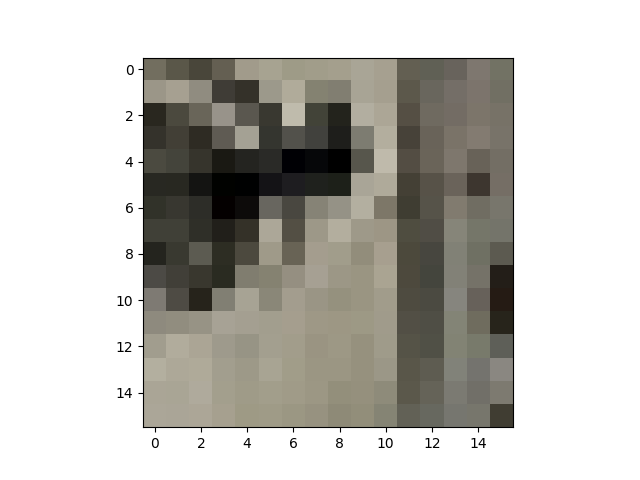
\includegraphics[width=.8\linewidth]{orig_patch.png}
  \caption{Original patch}
\end{subfigure}%
\begin{subfigure}{.5\columnwidth}
  \centering
  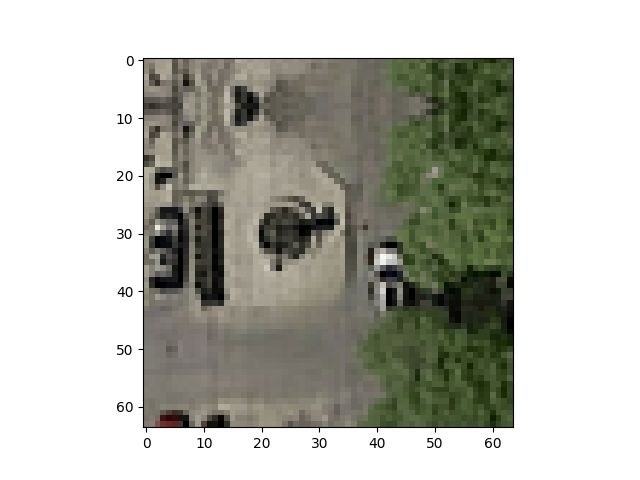
\includegraphics[width=\linewidth]{cont_added_patch.png}
  \caption{Context added patch}
\end{subfigure}
\caption{Context augmentation for patches}
\label{fig:patches}
\end{figure}

The patch size was determined empirically by trying out different context-added
sizes. We found that a context-added patch size of 64 provided the best score
on the Kaggle
competition\footnote{\url{inclass.kaggle.com/c/cil-road-segmentation-2017}}.

\subsection{Class balancing}
\label{sec:balance}
Training with a balanced dataset (i.e., a dataset with an equal number of
patches of each class) helps reduce the bias towards a certain value in the
form of a prior, which is due to the error minimization we are performing.
Because the provided input dataset was highly unbalanced (i.e., the number of
background patches was approximately three times greater than the number of
road patches), we balanced the data by randomly choosing a limited number of
background patches to train with. 


\section{Models and Methods}
\label{sec:model_and_methods}
\subsection{Baseline Model}
The baseline model works on batches of $16 \times 16$ patches.\\
 Its configuration is as follows:
 $IN(3, 16\times16)
-C(32, 5\times5 /1) - MP(2 / 2) - C(64, 5\times5 /1) - MP(2 / 2)
-FC(512)-FC(2)$\\
Where:
\begin{itemize}
\item $IN(a,b\times c)$ -- Input image of $a$ channels and size $b \times  c$
\item $CONV(a,b\times c / d)$ -- Convolution layer with depth $a$, window size $b\times c$ and stride $d$
\item $FC(a)$ -- Fully Connected layer of size $a$
\item $MP(a / b)$ -- Max Pooling layer of size $a$ with stride $b$
\end{itemize}

The weights of the network are L2 regularized and the optimizer used is the Momentum Optimizer  with an exponential decaying learning rate with a decay rate of 0.95 and starting at 0.01.
Each convolutional layer is followed by a rectified linear unit ($RELU$) and the activation function in the Fully Connected layers are the identity function .
In the end, the softmax function is applied to the output of the last Fully Connected layer. 
\subsection{Improved CNN Architecture}
The core of our work is the CNN design. We have got the main idea for the architecture
of the network from Alina Elena \cite{mthesis}. In this design, they connect both a VGG network \cite{vgg} and an AlexNet network \cite{alexnet} to create a dual stream network that takes as input the local patch to be predicted and the whole image as context.
Our solution takes this network as inspiration, however it only takes the local information as input. This decision was done due to limited data and also because empirically the results obtained with it were good.

Our CNN network can be described as follows: \\
$IN(3, 64\times64)
-C(64, 3\times3 /2) - MP(2 / 2) - C(128, 3\times3 /2) - MP(2 / 2)
-C(256, 3\times3 /2) - MP(2 / 2) - C(512, 3\times3 /2) - MP(2 / 2)
-FC(2048)-FC(2048)-FC(2)$\\

Additionally all convolutional layers are followed by rectified linear units ($RELU$) layer. The output of the CNN is the softmax function for the two classes and we use the Adam optimizer \cite{adam}.

To reduce overfitting, we initialize the parameters of the network using xavier's initialization algorithm \cite{xavier} and we also use a dropout rate of 0.5 on all the Fully Connected layers during training.
\subsection{Error function}
Our CNN model reduces the log-loss, but for the evaluation we have used two other loss metrics. The first one was
the classification error and it was used on the validation set that helped us find the right number of training epochs. 
Further discussion on that will follow in the next section. The second one was the F-1 score to calculate
the test error. The latter was given by the Kaggle competition.


\subsection{Model hyper-parameters}
Since we used the Adam optimizer, there were not many parameters to tune. One parameter was the batch size, which we 
have not changed from the baseline model since in the one of previous exercises we have learned the it should nether be too
big nor too small, so we found 32 to be a good choice. The only other parameter to tune was the number of training epochs.
This one we have empirically chosen to be 300 based on training the model on 95\% of the images and 
validating it in every epoch on the remaining 5\% of the images. The Figure \ref{fig:loss} shows
how the validation error changes with the number of epochs. Beside these, there were no further hyper-parameters to tune.


\begin{figure}[h]
 \centering
  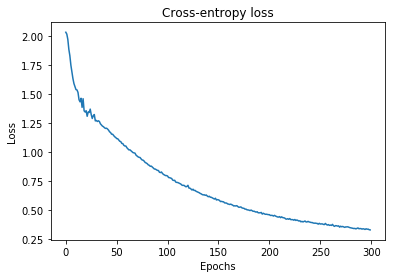
\includegraphics[width=.8\linewidth]{loss.png}
  \caption{Cross entropy loss with 5\% validation set}
  \label{fig:loss}
\end{figure}

\subsection{Post-processing}
In order to improve the output obtained from the CNN network, we perform a post-processing step that helps reduce the noise of the output image and correct some prediction errors. Errors may appear in the image due to the inconsistencies in the roads. As an example, objects that overlap with roads such as cars or trees might have a negative effect on the classification due to their difference in color and shape in contrast with the road. Furthermore, structures like rooftops might sometimes appear like roads.\\
\subsubsection{Model Description}
We propose an approach that first denoises the image and then performs a prediction on the patches. Given the output of the CNN as a grayscale image, we perform a denoising using wavelets. Following the denoising, we convert the image to binary representation (either black or white patches) and then we perform a prediction of the \textit{border patches} using a Multilayer Perceptron (MLP). We tried other models such as SVM (or SVC for classification) and Random Forest, however we obtained the best results with the MLP. Finally, we change the patch's color if at least 7 out of 8 neighbors have a different color, because we believe that it is highly likely that it is a misclassified patch.

In figure \ref{fig:denoising} we can see the outputs of each step. We start with the raw CNN output, we then apply the wavelet denoising, and afterwards we apply the MLP to the border patches only and fill the patch color with the neighbouring technique.
\subsubsection{Wavelet denoising}
For the denoising, we choose wavelets because the results obtained were smooth and appropiate for road images. The wavelets used are Daubechies 1 wavelets. Furthermore the denoising is done assigning the hyperparameter sigma to 3. 
\subsubsection{Multilayer Perceptron classifier}
The input datapoints of the classifier are patches surrounded with context. For the patches, we consider a window of $11\times11$ patches, with the current one to be classified centered. Also, we do not classify all the patches in the image, only the \textit{border patches}. A patch is considered a \textit{border patch} if 5 of its 8 immediate neighbors have a distinct color. We only consider these patches because we observed that the other patches are generally correctly classified as the raw output of the CNN is not so noisy compared to the baseline's output.\\
For the structure of the classifier itself, the parameters were found using a cross validated grid search. The best settings found are to use two hidden layers of size 50 each and to use the logistic activation function. Finally the training of the MLP was done on the 309 groundtruth images that we obtain using data augmentation techniques.

\begin{figure}
\centering
\begin{subfigure}{.3\columnwidth}
  \centering
  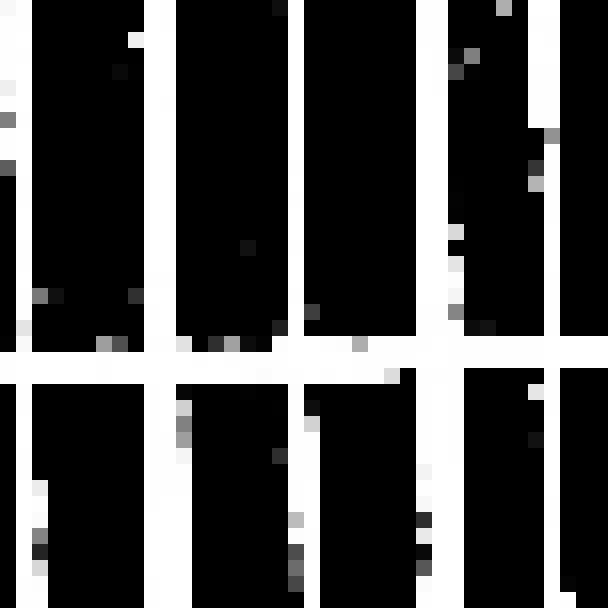
\includegraphics[width=.8\linewidth]{output_cnn_raw.png}
  \caption{Raw CNN output}
\end{subfigure}%
\begin{subfigure}{.3\columnwidth}
  \centering
  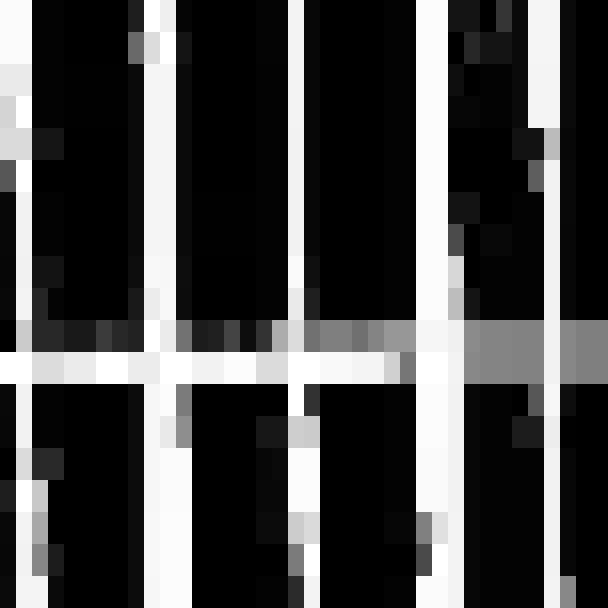
\includegraphics[width=.8\linewidth]{only_wav.png}
  \caption{Wavelet denoising}
\end{subfigure}
\begin{subfigure}{.3\columnwidth}
  \centering
  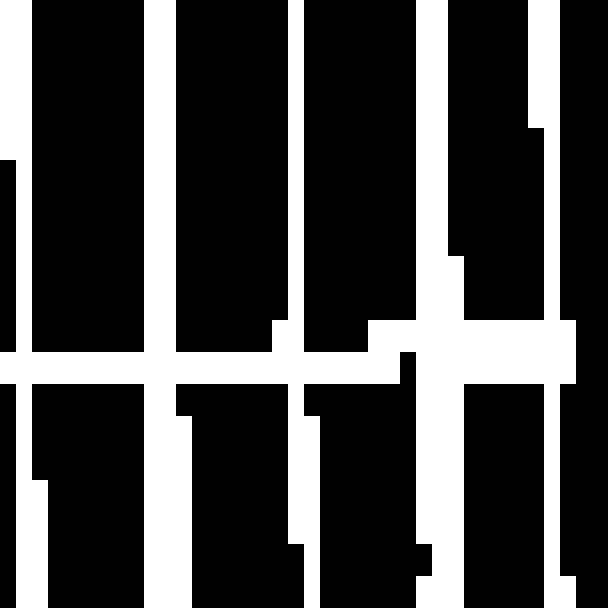
\includegraphics[width=.8\linewidth]{final_res.png}
  \caption{Wavelet + MLP + Neighbor}
\end{subfigure}
\caption{Post-Processing steps}
\label{fig:denoising}
\end{figure}


\section{Results}
\label{sec:results}
\subsection{Implementation}
The model presented here is implemented using tensorflow for the CNN and the denoising was developed using scikit-learn. The CNN was trained on an Microsoft Azure NV6 instance for 20 hours and 52 minutes using one kernel of the Nvidia Tesla m60 GPU using 2048 CUDA cores provided by the instance. Furthermore the post-processing part was also trained on the Azure instance. The training of the MLP using 6 jobs was done in 2 hours and 51 minutes for the Grid Search method in order to find the optimal parameters.
\subsection{Score}
The raw output of our CNN achieves an F1 score of $\sim 0.9$. With post-processing, we aim to achieve a higher score and to fix some classification errors. After denoising, the score achieved is $\sim 0.9095$. From the score, we can see how the results obtained from the CNN network have already a relatively high score and that post-processing does not help significantly to improve the score. The solutions are close to the state-of-the-art methods, however they can be improved by extending the training time as can be seen in figure \ref{fig:loss}.

\subsection{Comparison to baseline model}
The baseline model achieves an F1 score of 0.73723 on the public Kaggle competition, which is significantly lower than the one obtained by our model. Furthemore, the output images obtained by the baseline model are noisy, with patches of roads completely isolated which is something that does not happen on roads.


\section{Conclusions}
\label{sec:conclusions}
In this paper we have discussed a novel method to solve road segmentation on satellite images. The relatively deep CNN presented seems to be a good compromise between ease of train for small dataset and accuracy. Furthermore, post-processing is an important step for road segmentation. The prior knowledge of the input images (roads), allows the training of models for image denoising that take into account the overall shape of the roads.\\
Regarding the score, despite the lack of input data it achieves in general high score close to state-of-the-art methods. However this could be improved by making the network more deep and with a further increase in the dataset, something which is left as an idea for further work.




\bibliographystyle{IEEEtran}
\bibliography{howto-paper}
\end{document}
